\documentclass[12pt,3p]{article}
\usepackage[T1]{fontenc}
\usepackage[utf8]{inputenc}
\usepackage[english]{babel}
\usepackage[margin=0.75in]{geometry}
\usepackage{amsmath}
\usepackage{mathtools}
\usepackage{enumitem}
\usepackage{physics}
\usepackage{bm}
\usepackage[font=small]{caption}
\usepackage{xcolor}


\usepackage[round,numbers]{natbib}
\usepackage[colorlinks = false]{hyperref}

\begin{document}

\title{\Large{FEniCS: Time Dependent Heat Equation} \vspace{-2ex}}
\author{Ida Ang, Edited \today}
\date{\vspace{-5ex}}
\maketitle

\tableofcontents
\newpage
%=====================================================================
%=====================================================================
%=====================================================================
\section{Problem Definition}
\vspace{-2ex}
This document references A Gallary of finite element solvers, \href{https://fenicsproject.org/pub/tutorial/html/.\_ftut1006.html}{the heat equation}. Some of the text is taken from either the documentation online or the code, but the goal of this document is to provide more details of the theory and conversion from the strong form, or partial differential equations, to the weak form, or integral equation. This document provides the detailed steps for beginners who might have just been exposed to indicial notation. In direct notation, bolded uncapitalized notation refers to vectors, unbolded notation refers to scalar variables.
 
%=====================================================================
%=====================================================================
%=====================================================================
\section{Formulations}
\vspace{-2ex}
The simplest formulation for Poisson's problem involves solving for one variable, $u$, which is known as a scalar field of scalar potential. The Poisson's equation shows up in many contexts, and the variable $u$ could be the concentration of some chemical solute, as a function of position x, or the temperature $T$ in some heat conducting medium. Classically, the equation can be referred to as the divergence of the gradient of some scalar field which then returns a scalar, some source term $f$.
\begin{subequations}\label{EqPoisson}
\begin{align}
\nabla \cdot \nabla u = \nabla^2 u = \Delta u = f \quad \text{in } \Omega 
\end{align}
\end{subequations}

It can also be referred to as the Laplacian of the variable field, where several notations are listed in Eq. \ref{EqPoisson}.
As an extension of the Poisson problem, which can be used to describe the stationary distribution of heat in a body, we can consider the time-dependent heat equation (or time-dependent diffusion equation), which describes the distribution of heat in a body over time. 
\begin{subequations}
\begin{align}
\frac{\partial u}{\partial t} & =\nabla^2 u+f \quad \text { in } \Omega \times(0, T], \\
u & =u_{\mathrm{D}} \quad \text { on } \partial \Omega \times(0, T] \\
u & =u_0 \quad \text { at } t=0 .
\end{align}
\end{subequations}
where in this particular problem, the Dirichlet boundary condition consists of the full boundary, $\partial \Omega = \Gamma_D$, and there is no Neumann boundary condition. The Dirichlet boundary condition (BC) is the essential boundary condition applied within the function space. Recall, that the Neumann boundary condition can be stated as in Eq. \ref{EqNeumannBC},
\begin{subequations}\label{EqNeumannBC}
\begin{align}
\nabla u \cdot \mathbf{n} = \pdv{u}{\mathbf{n}} &= g \quad \quad \quad \text{on } \Gamma_N \\
\pdv{u}{x_i} n_i  &= g
\end{align}
\end{subequations}
where it is the natural boundary condition which is subsumed into the variational weak form. The source term $f$  can be defined as follows:
\begin{equation}\label{EqSourceTerm}
f(x,y, t) = 1 + x^2 + \alpha y^2 + \beta t
\end{equation} 
In order to obtain the weak form, 1) multiply the strong form with a test function, 2) Integrate over the domain of interest, and 3) use integration by parts. 
\begin{align}\label{EqBefIntParts}
\int_{\Omega} \frac{\partial u}{\partial t} v \, dv = \int_{\Omega} \pdv[2]{u}{x} v \, dv + \int_{\Omega} f v \, dVv
\end{align}
Use integration by parts,
\begin{equation}\label{EqIntParts1}
(fg)' = f'g + fg' \rightarrow f'g = (fg)' - fg' \rightarrow f''g = (f'g)' - f'g'
\end{equation}
Where we can substitute $f'' = \pdv[2]{u}{x_i} $ and $g = v$ into Eq. \ref{EqIntParts1}
\begin{equation*}
\pdv[2]{u}{x} v = \nabla \cdot \bigg( \pdv{u}{x} v \bigg) - \pdv{u}{x} \pdv{v}{x}
\end{equation*}
Substitute into Eq. \ref{EqBefIntParts}
\begin{align*}
\int_{\Omega} \frac{\partial u}{\partial t} v \, dv
	&= \int_{\Omega} \pdv[2]{u}{x} v \, dv + \int_{\Omega} f v \, dv \\
\int_{\Omega} \frac{\partial u}{\partial t} v \, dv 
	&= \int_{\Omega} \nabla \cdot \bigg( \pdv{u}{x} v \bigg) \, dv - \int_{\Omega} \pdv{u}{x} \pdv{v}{x} \, dv
	  + \int_{\Omega} f v \, dv \quad \text{Divergence Theorem} \\
\int_{\Omega} \frac{\partial u}{\partial t} v \, dv
	&= \int_{\partial \Omega} \bigg( \pdv{u}{x} \cdot \mathbf{n} \bigg) v \, ds 
	- \int_{\Omega} \pdv{u}{x} \pdv{v}{x} \, dv + \int_{\Omega} f v \, dv \\
\int_{\Omega} \frac{\partial u}{\partial t} v \, dv 
	&= \int_{\partial \Omega} g v \, ds - \int_{\Omega} \pdv{u}{x} \pdv{v}{x} \, dv + \int_{\Omega} f v \, dv
\end{align*}
Therefore, the weak form in  direct notation
\begin{equation}\label{EqWeakForm}
\int_{\Omega} \frac{\partial u}{\partial t} v \, dv + \int_{\Omega} \nabla u \cdot \nabla v \, dv
	= \int_{\Omega} f \cdot v \, dv + \int_{\Gamma_N} g \cdot v \, ds 
\end{equation}

%=====================================================================
%=====================================================================
\subsection{Time Integration}
\vspace{-1ex}
The time derivative can be discretized by a finite difference approximation, where the following approximation is given for a backwards difference at time $t_{n+1}$
\begin{equation}\label{EqFiniteDiff}
\left(\frac{\partial u}{\partial t}\right)^{n+1} \approx \frac{u^{n+1}-u^n}{\Delta t}
\end{equation}
where we can substitute Eq. \ref{EqFiniteDiff} into Eq. \ref{EqWeakForm} at time $t_{ n+1}$
\begin{align*}
\int_{\Omega} \left( \frac{\partial u}{\partial t} \right)^{n+1} v \, dv 
+ \int_{\Omega} \nabla u^{n+1} \cdot \nabla v \, dv
	= \int_{\Omega} f^{n+1} \cdot v \, dv + \int_{\Gamma_N} g^{n+1} \cdot v \, ds \\
\int_{\Omega} \frac{u^{n+1}-u^n}{\Delta t} v \, dv 
+ \int_{\Omega} \nabla u^{n+1} \cdot \nabla v \, dv
	= \int_{\Omega} f^{n+1} \cdot v \, dv + \int_{\Gamma_N} g^{n+1} \cdot v \, ds \\
\int_{\Omega} \big( u^{n+1}-u^n \big) v \, dv 
+ \Delta t \, \int_{\Omega} \nabla u^{n+1} \cdot \nabla v \, dv
	= \Delta t \, \int_{\Omega} f^{n+1} \cdot v \, dv + \Delta t \, \int_{\Gamma_N} g^{n+1} \cdot v \, ds 
\end{align*}
where we assume $u^n$ is a quantity from the previous time step, $t_n$, while we are computing the solution at time $t_{n+1}$; therefore, we can introduce $u$ instead of $u^{n+1}$, etc. giving the following equation.
\begin{align}\label{EqTimeDiscrete}
\int_{\Omega} \big( u -u^n \big) v \, dv 
+ \Delta t \, \int_{\Omega} \nabla u \cdot \nabla v \, dv
	= \Delta t \, \int_{\Omega} f \cdot v \, dv + \Delta t \, \int_{\Gamma_N} g \cdot v \, ds 
\end{align}
Eq. \ref{EqTimeDiscrete} is the general form, but for our specific problem there is no Neumann boundary condition leading to the following equation. 
\begin{align}\label{EqTimeDisSpec}
\int_{\Omega} \big( u -u^n \big) v \, dv 
+ \Delta t \, \int_{\Omega} \nabla u \cdot \nabla v \, dv
	= \Delta t \, \int_{\Omega} f \cdot v \, dv 
\end{align}

%=====================================================================
%=====================================================================
%=====================================================================
\section{FEniCS Implementation}
\vspace{-2ex}
Just as in the prior section, the variable $u$ is used for the unknown value at time step $t_{n+1}$ for the unknown $u^{n+1}$ and the variable u\_n is used for $u^n$ at the previous (known) time step. The initial value of u\_n can be computed by either projection or interpolation of $u_0$, which in this case is defined with the expression in Eq. \ref{EqSourceTerm} \\
{\fontfamily{qcr}\selectfont
u\_D = Expression('1 + x[0]*x[0] + alpha*x[1]*x[1] + beta*t',  \\
\indent \indent \indent \indent \indent \indent \indent degree=2, alpha=alpha, beta=beta, t=0) \\ \\
}
Note, to recover the exact solution to machine precision, it is important to compute the discrete initial condition by interpolating $u_0$, which ensures that the degrees of freedom are exact (to machine precision) at t=0. \textcolor{red}{Projection results in approximate values at the nodes.} The syntax for either of these commands are included below. \\
{\fontfamily{qcr}\selectfont
u\_n = interpolate(u\_D, V) \\
u\_n = project(u\_D, V) \\ \\
}
Equation \ref{EqTimeDisSpec} can be stated by moving all the variables to the left hand side of the equation and letting FEniCS determine the bilinear and linear forms. \\
{\fontfamily{qcr}\selectfont
F = u*v*dx + dt*dot(grad(u), grad(v))*dx - (u\_n + dt*f)*v*dx \\
a, L = lhs(F), rhs(F) \\ \\
}
Within the loop, the problem an be solved for each time step. For verification, the expression can be interpolated into the function space as the exact solution u\_e. The error can be computed and saved to an array called {\fontfamily{qcr}\selectfont PostTxt} which is then saved to a text file for plotting in {\fontfamily{qcr}\selectfont PostProc.py} \\
{\fontfamily{qcr}\selectfont
PostTxt = np.zeros((NumSteps, 3)) \\
for n in range(NumSteps): \\
\indent     solve(a == L, u, bc) \\
\indent  u\_e = interpolate(u\_D, V) \\
\indent  error = np.abs(u\_e.vector() - u.vector()).max() \\
\indent PostTxt[n, :] = np.array([n, t, error]) \\
\indent np.savetxt(Dir + '/PostProc.txt', PostTxt) \\ \\
}
Lastly, the proper variables must be updated. Inside the time loop, observe that u\_D.t must be updated to enforce computation of Dirichlet conditions at the next time step. A Dirichlet condition defined in terms of an Expression looks up and applies the value of a parameter such as t when it gets evaluated and applied to the linear system. Furthermore, we must assign the new computed solution u to the variable u\_n (previous). If we set u\_n = u, the u\_n variable will be the SAME variable as u, but we need two values, one for the previous and current time step.\\
{\fontfamily{qcr}\selectfont
for n in range(NumSteps): \\
\indent t += dt \\
\indent u\_D.t = t  \\
\indent  u\_n.assign(u) 
}

\newpage
\section{Results}
\vspace{-2ex}
Snapshots of the simulation for $N_x = N_y = 100$ are included in Fig. \ref{FigScreenshots}. 

\begin{figure*}[!htb]
\centering
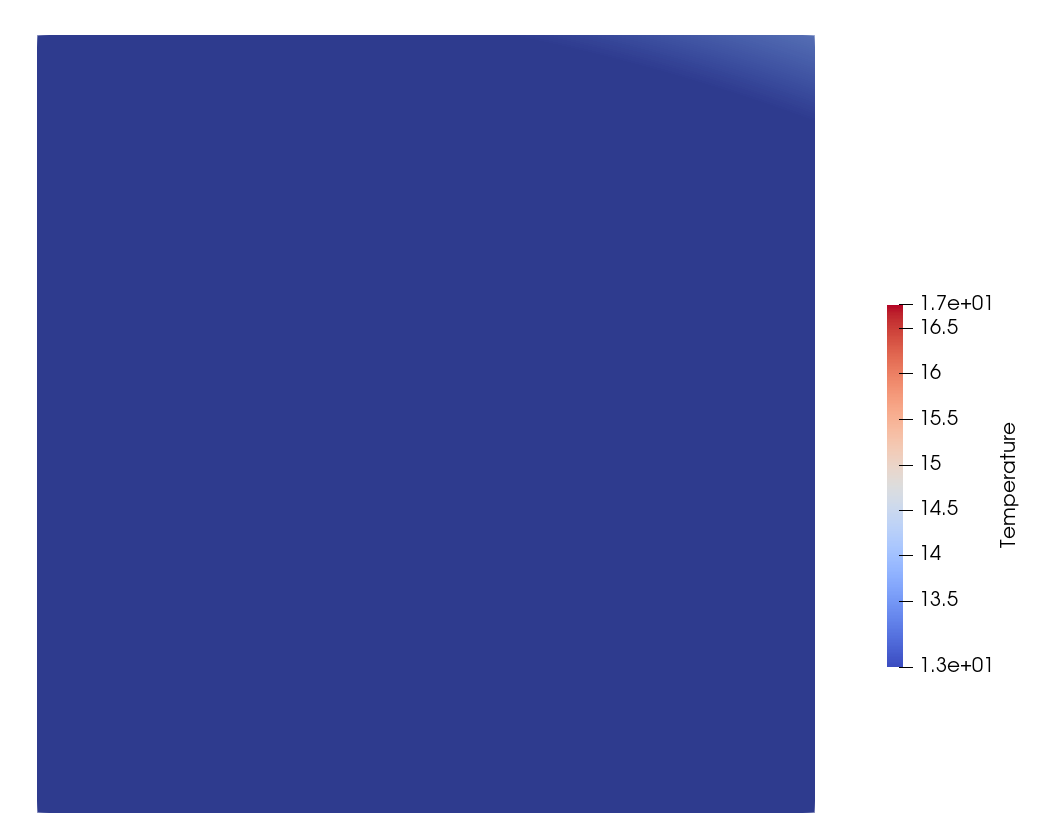
\includegraphics[width=0.3\textwidth]{./Results/Interpolate/S_50_N_100/TempCrop/Temp_35}
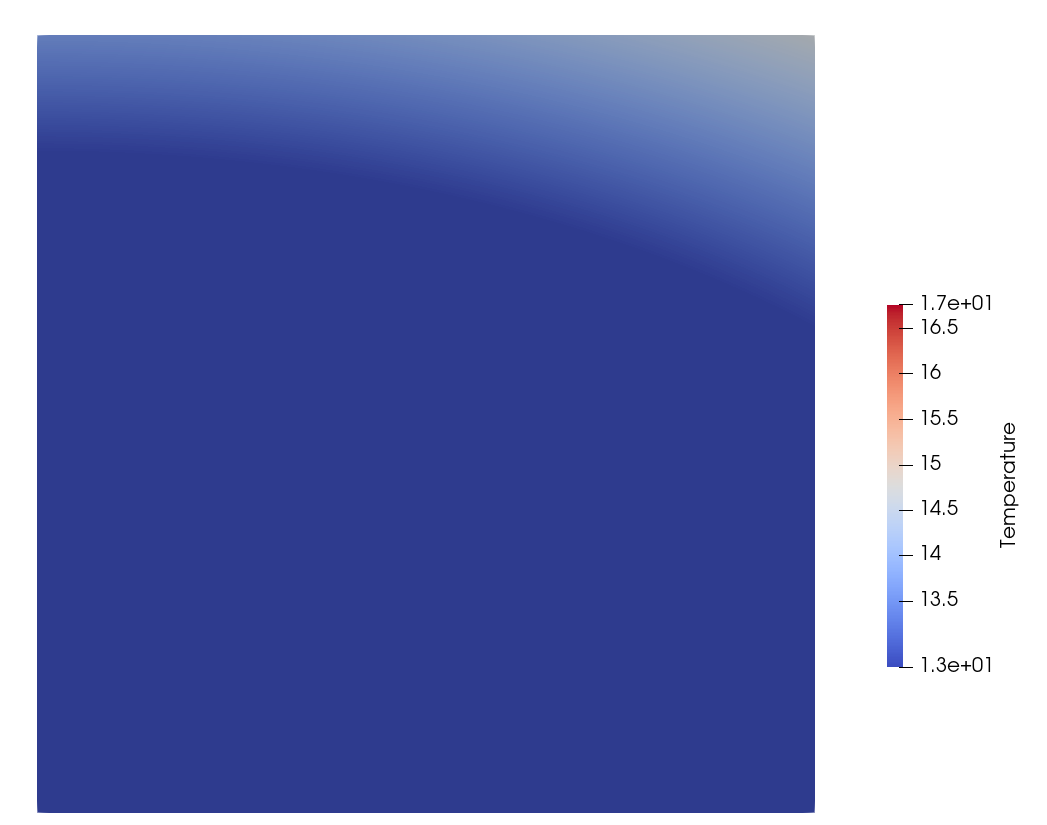
\includegraphics[width=0.3\textwidth]{./Results/Interpolate/S_50_N_100/TempCrop/Temp_40} 

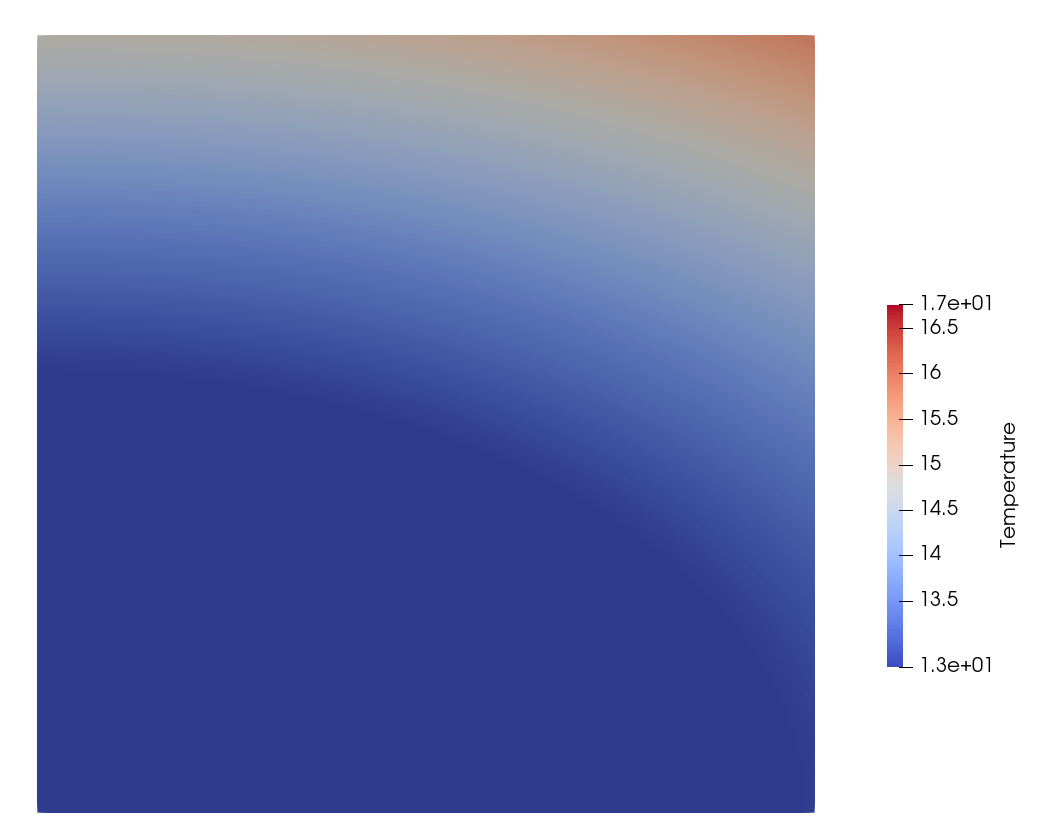
\includegraphics[width=0.3\textwidth]{./Results/Interpolate/S_50_N_100/TempCrop/Temp_45}
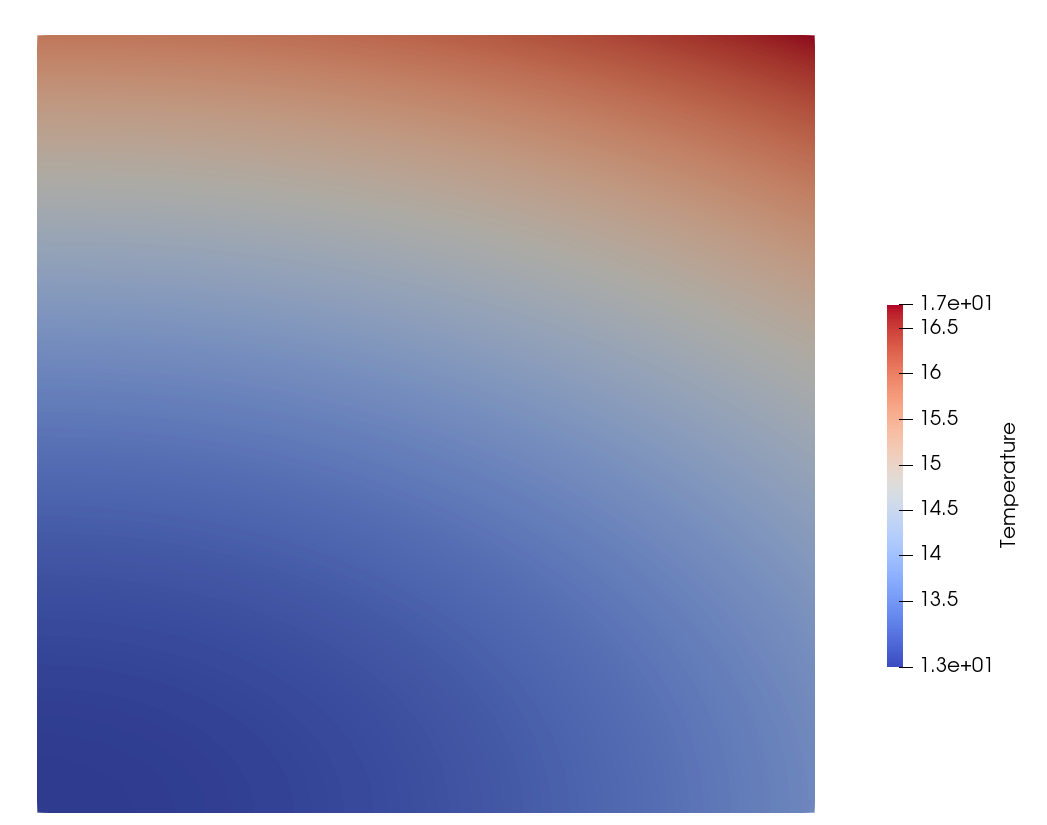
\includegraphics[width=0.3\textwidth]{./Results/Interpolate/S_50_N_100/TempCrop/Temp_49}
\caption{Temperature at step 35, 40, 45, and 49 for $\Delta t = 0.2$}
\label{FigScreenshots}
\end{figure*}

Fig. \ref{FigCompErrorInt} demonstrates the error over the course of the simulation steps and simulation time for different mesh resolutions using the {\fontfamily{qcr}\selectfont
interpolation} command, while Fig. \ref{FigCompErrorProj} demonstrates the same except the {\fontfamily{qcr}\selectfont project} command is used. 

\begin{figure*}[!htb]
\centering
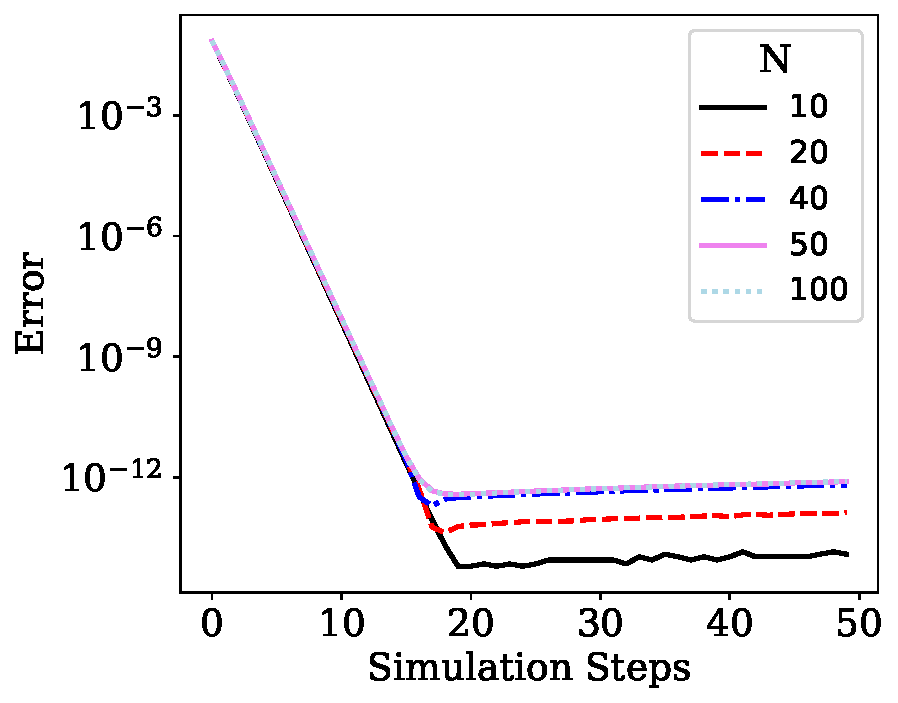
\includegraphics[width=0.45\textwidth]{./Images/CompIntSimSteps}
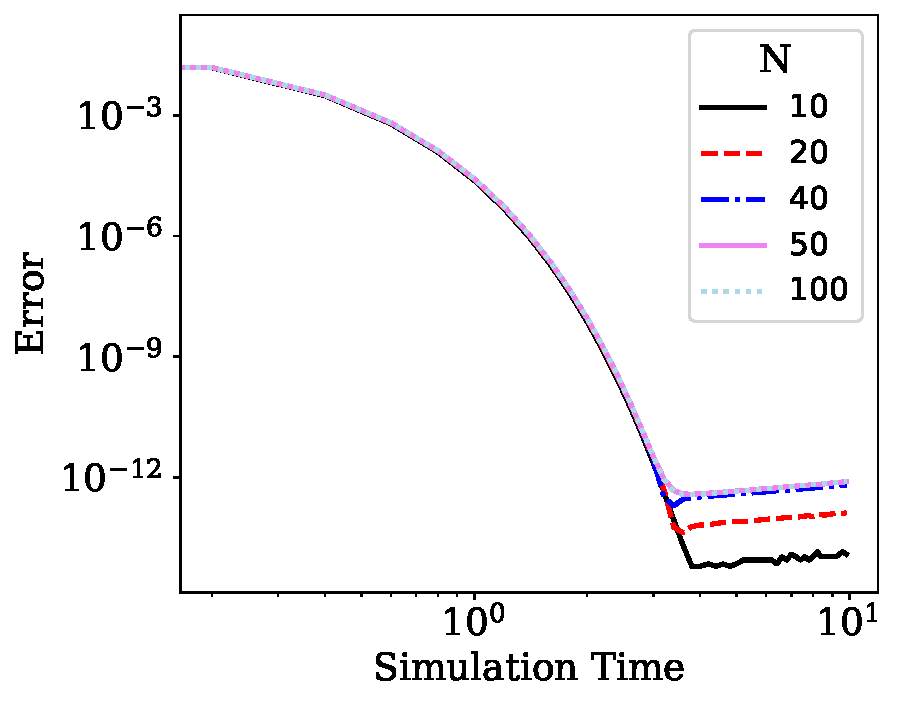
\includegraphics[width=0.45\textwidth]{./Images/CompIntSimTime}
\caption{ Error plotting for different mesh resolutions using the interpolation command.}
\label{FigCompErrorInt}
\end{figure*}

There is no discernible difference in the error from these plots, and the error is relatively low and demonstrates small but negligible differences between the computation and exact solution. 

\begin{figure*}[!htb]
\centering
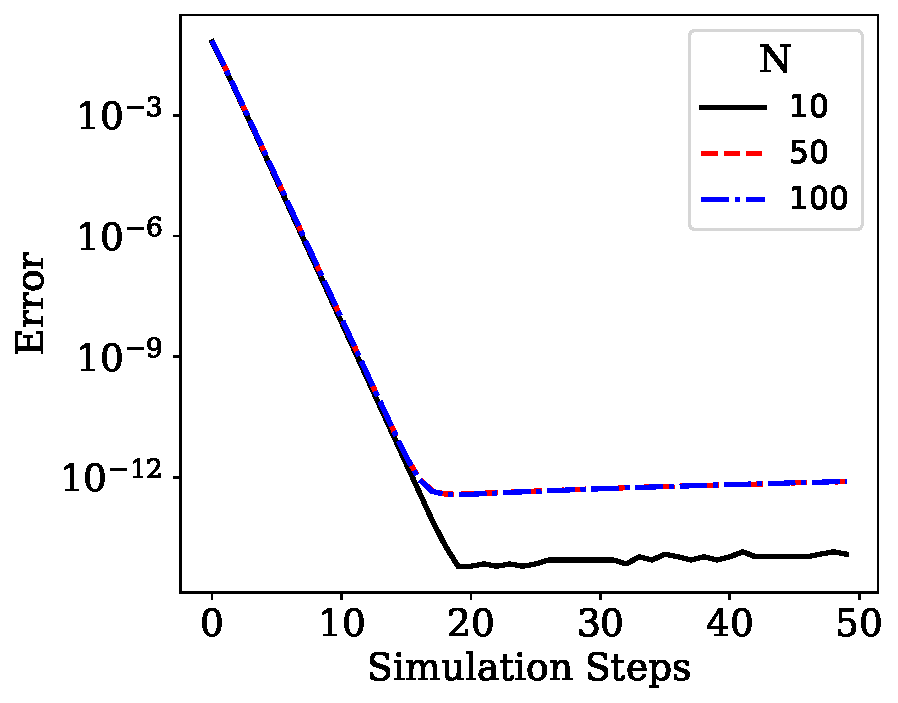
\includegraphics[width=0.45\textwidth]{./Images/CompProjSimSteps}
\includegraphics[width=0.45\textwidth]{./Images/CompProjSimtime}
\caption{ Error plotting for different mesh resolutions using the project command.}
\label{FigCompErrorProj}
\end{figure*}



\end{document}
